\section{Unicode}

\subsection{Computers and Writing Systems}

Here's the unfortunate truth: computers can only read, write, or think in 1s and
0s. Any text that a computer deals with must somehow be stored as a number;
encoding schemes describe how the computer should convert this number into a
string of characters or vice versa. All computers on a network must adhere to
the \textit{same} encoding system, lest streams of text be interpreted
incorrectly and communication failures ensue.

The American Standard Code for Information Interchange (ASCII), a 7-bit encoding
scheme, was released in 1963 and quickly became the worldwide standard for
digital text encoding. It was even endorsed by President Lyndon Johnson, who
ordered in 1968 that all federal government computers must be ASCII-compatible.
This was a easy decision for the US President, as the 128 ($2^7$) characters in ASCII
included all necessary symbols to represent modern English text.

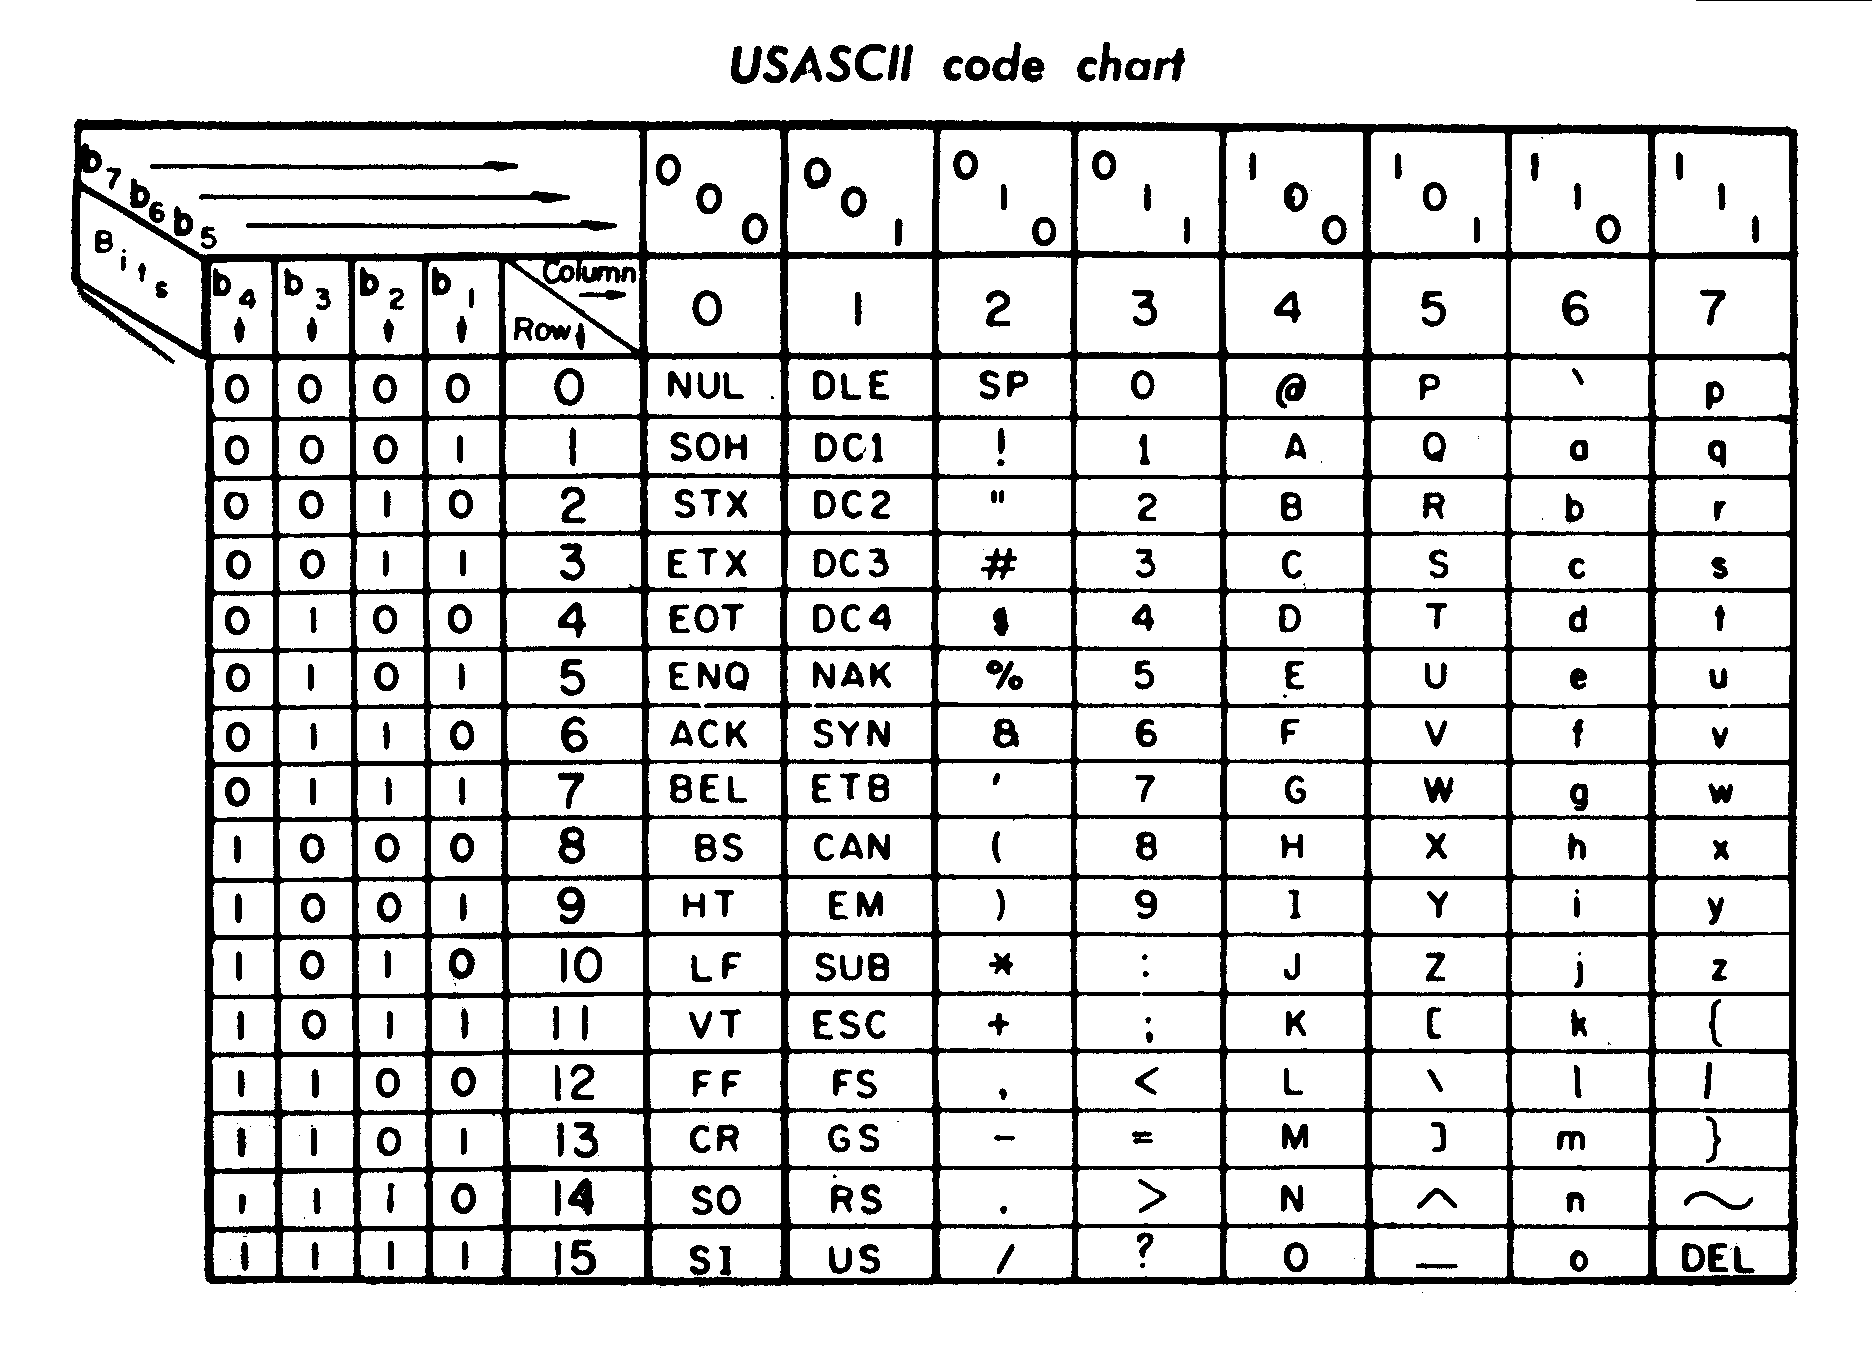
\includegraphics[scale=0.1]{subtex/ascii-chart.png}

The problem arose when computer technology spread beyond the labs of Silicon
Valley and government offices in Washington. In other countries and languages,
there was a vast array of linguistic forms, including diacritical marks,
right-to-left scripts, and pictographic writing systems, which ASCII was
unequipped to handle. In the 1990s, many national encoding schemes were created
to represent languages other than English. Most of these were 8-bit "extensions"
of ASCII of 256 characters ($2^8$) , meaning the original 128-character ASCII
set remained intact, and useful non-English characters were added in the
remaining slots. The only problem here is that they were not intercompatible,
meaning that documents might not "play nice" when transferred between countries
or languages.

Unicode and its dominant encoding scheme UTF-8 intend to alleviate these
problems by collecting all of the world's glyphs into one system. The 127
characters in ASCII are represented using the same single-byte codes, which
means that no conversion for existing ASCII files is necessary, and these will
not become bloated in a new conversion scheme. But the encoding scheme takes
advantage of modern computer's greater storage capacities to represent 1,112,064
distinct characters. 
